\documentclass[11pt, english, letterpaper]{article}
\usepackage[T1]{fontenc}
\usepackage{textcomp}
\usepackage{lmodern}
\usepackage{graphicx}
\usepackage{csquotes}
% \usepackage[nolists,
%             heads,
%             nomarkers,
%             figuresfirst,
%             nofighead,
%             notabhead]{endfloat}
\usepackage[authordate,
            backend=biber,
            hyperref=true,
            maxcitenames=2]{biblatex-chicago}
\usepackage{etoolbox}
\usepackage[usenames,dvipsnames,table]{xcolor}
\usepackage[margin=1in]{geometry}
\usepackage{epstopdf}
\usepackage{babel}
\usepackage{gensymb}
\usepackage{multicol}
\usepackage{caption}
\usepackage{subcaption}
\usepackage{amsmath}
\usepackage{bm}
\usepackage{bbm}
\usepackage{breqn}
\usepackage{mathtools}
\usepackage{verbatim}
\usepackage[normalem]{ulem}
\usepackage{setspace}
\usepackage{xtab}  
\usepackage{float}
\usepackage[section]{placeins}
\usepackage{changepage}
\usepackage{tikz}
\usepackage{pgfplots}
\pgfplotsset{compat=1.18}
\usetikzlibrary{decorations.pathreplacing}
\usepackage{pgffor}
\usepackage{longtable}
\usepackage{threeparttable}
\usepackage{rotating}
\usepackage{tabulary}
\usepackage{booktabs}
\usepackage{pdflscape}
\usepackage{verse}
\usepackage[hang, flushmargin]{footmisc}
\usepackage[colorlinks = true,
            linkcolor = black,
            urlcolor  = black,
            citecolor = black,
            linkbordercolor = {white},
            anchorcolor = black]{hyperref}
\usepackage{footnotebackref}            
\usepackage[colorinlistoftodos,prependcaption]{todonotes}
\usepackage{xargs} 
\usepackage[document]{ragged2e}
\usepackage[affil-it]{authblk}
\usepackage{soul}
\usepackage{epigraph}


% %COMMENT OUT BELOW IF USING NON-RANDOM AUTHOR ORDER
%     \renewcommand\Authsep{ \textcircled{r} }
%     \renewcommand\Authands{ \textcircled{r} }
% %COMMENT OUT ABOVE IF USING NON-RANDOM AUTHOR ORDER

\linespread{1.6} % Spacing of lines 
\def\arraystretch{1.3} % Spacing of table rows 
\setlength{\tabcolsep}{4pt} % Spacing of table columns
\setlength{\epigraphwidth}{0.4\textwidth}

%------------------------------------------------- HEADER WARNING
\usepackage{fancyhdr}
\setlength{\headheight}{15.2pt}
\pagestyle{fancy}
\rhead{}
\lhead{}
% \chead{\color{red}{\textbf{PRELIMINARY DRAFT. DO NOT CITE OR CIRCULATE}}}
\renewcommand{\headrulewidth}{0pt}
%-------------------------------------------------|

\newcommand{\citep}{\parencite}

\newcommand{\attrib}[1]{%
\nopagebreak{\raggedleft\footnotesize #1\par}}
\renewcommand{\poemtitlefont}{\normalfont\large\itshape\centering}


% Make all the citation text hyperlinked. 
% Taken from: 
% https://groups.google.com/forum/#!topic/comp.text.tex/rSPhG2jd3Ks 
\DeclareCiteCommand{\cite}
  {\usebibmacro{prenote}}
  {\usebibmacro{citeindex}%
   \printtext[bibhyperref]{\usebibmacro{cite}}}
  {\multicitedelim}
  {\usebibmacro{postnote}}

\DeclareCiteCommand*{\cite}
  {\usebibmacro{prenote}}
  {\usebibmacro{citeindex}%
   \printtext[bibhyperref]{\usebibmacro{citeyear}}}
  {\multicitedelim}
  {\usebibmacro{postnote}}

\DeclareCiteCommand{\parencite}[\mkbibparens]
  {\usebibmacro{prenote}}
  {\usebibmacro{citeindex}%
   \printtext[bibhyperref]{\usebibmacro{cite}}}
  {\multicitedelim}
  {\usebibmacro{postnote}}

\DeclareCiteCommand*{\parencite}[\mkbibparens]
  {\usebibmacro{prenote}}
  {\usebibmacro{citeindex}%
   \printtext[bibhyperref]{\usebibmacro{citeyear}}}
  {\multicitedelim}
  {\usebibmacro{postnote}}

\DeclareCiteCommand{\footcite}[\mkbibfootnote]
  {\usebibmacro{prenote}}
  {\usebibmacro{citeindex}%
   \printtext[bibhyperref]{\usebibmacro{cite}}}
  {\multicitedelim}
  {\usebibmacro{postnote}}

     
\DeclareCiteCommand{\citeauthor}
  {\boolfalse{citetracker}%
   \boolfalse{pagetracker}%
   \usebibmacro{prenote}}
  {\indexnames{labelname}%
   \printtext[bibhyperref]{\printnames{labelname}}}
  {\multicitedelim}
  {\usebibmacro{postnote}}
  
\DeclareCiteCommand{\citeyear}
  {\boolfalse{citetracker}%
   \boolfalse{pagetracker}%
   \usebibmacro{prenote}}
  {\printtext[bibhyperref]{\printfield{year}}}
  {\multicitedelim}
  {\usebibmacro{postnote}}
  
\renewbibmacro*{cite:label}{%
  \iffieldundef{label}
    {\printfield[citetitle]{labeltitle}}
    {\printfield{label}}}

\renewbibmacro*{cite:year+labelyear}{%
  \iffieldundef{year}
    {}
    {\printfield{year}%
     \printfield{labelyear}}}

\renewbibmacro*{cite:shorthand}{%
  \printfield{shorthand}}


% Make the font in the reference list small 
\renewcommand*{\bibfont}{\footnotesize}
% Reduce space between references 
\setlength\bibitemsep{0pt}

%Define todo shortcuts
\newcommandx{\cc}[2][1=]{\todo[linecolor=Tan,backgroundcolor=Tan!25,bordercolor=Black,#1]{#2}}
\newcommandx{\CITE}[2][1=]{\todo[linecolor=cyan,backgroundcolor=cyan!25,bordercolor=Black,#1]{cite}}
\newcommandx{\unsure}[2][1=]{\todo[size=\tiny,linecolor=red,backgroundcolor=red!25,bordercolor=red,#1]{#2}}
\newcommandx{\change}[2][1=]{\todo[size=\tiny,linecolor=blue,backgroundcolor=blue!25,bordercolor=blue,#1]{#2}}
\newcommandx{\info}[2][1=]{\todo[size=\tiny,linecolor=OliveGreen,backgroundcolor=OliveGreen!25,bordercolor=OliveGreen,#1]{#2}}
\newcommandx{\improve}[2][1=]{\todo[size=\tiny,linecolor=Plum,backgroundcolor=Plum!25,bordercolor=Plum,#1]{#2}}


\addbibresource{references.bib}
% Strip the month and day from the citation data
\AtEveryBibitem{%
  \clearfield{day}%
  \clearfield{month}%
  \clearfield{endday}%
  \clearfield{endmonth}%
  \clearlist{language}%
}
\AtEveryCitekey{%
  \clearfield{day}%
  \clearfield{month}%
  \clearfield{endday}%
  \clearfield{endmonth}%
  \clearlist{language}%
}


% % to put citations in numbers and italics (a la sceince)
% \usepackage[round, numbers, sort&compress]{natbib}
% \bibliographystyle{ieeetr}
% \setcitestyle{citesep={,}} 
% \renewcommand{\citenumfont}[1]{\textit{#1}}

% Latex is not happy with \input in tables 
\makeatletter
\newcommand*\ExpandableInput[1]{\@@input#1 }
\makeatother

\def\sym#1{\ifmmode^{#1}\else\(^{#1}\)\fi}

\newcommand*{\tabPath}{placeholder}%
\newcommand*{\rootPath}{paper/}


\begin{document}
\justifying

% Title ideas 
% Beavers over Brexit
% Beavers or Brexit
% Bigger than Brexit?

\vspace{-2em} 

\title{Bigger than Brexit? \\ Estimating the impact of wildlife reintroduction on land use\thanks{Acknowledgments: I am grateful to Eyal Frank for invaluable feedback.}}
% People to recognize:
% Eyal, other readers (Tai, Seth)
% Data providers: NatureScot, AgriStats 
% I thank the participants of [discussions] for helpful comments. I acknowledge the generous provision of data by [data providers].}
\author[1]{\small Miriam Gold}

\affil[1]{\footnotesize Energy Policy Institute at Chicago, University of Chicago}
\date{\today}
\maketitle

\begin{center}
\vspace{-3em}
\textbf{\textcolor{red}{Preliminary draft. Do not circulate without permission.}}
\end{center}

\begin{abstract}
    \singlespacing 
    Natural capital, including wildlife, is widely understood to enter the production function. Ex-ante, agents may not know its effect on productivity, leading risk-averse operators to neutralize threats before the true effect is known. In the case of wildlife management, such action may be welfare reducing if it degrades ecosystem function, reduces biodiversity, or eliminates beneficial services provided by culled animals. There remains, however, little empirical evidence on the counterfactual partial production function effect of so-called ``nuisance'' species in the absence of control operations. The beaver (\textit{Castor fiber}), despite producing well-documented benefits as an ecosystem engineer, can hinder agricultural productivity by inundating fields, grazing crops, felling trees, and collapsing flood banks. A recent unauthorized reemergence of beavers in Scotland, where they had been driven extinct centuries earlier, has triggered a backlash among agricultural producers, with some claiming the impacts on their industry would be greater than those of Brexit. Using a series of comprehensive regional surveys conducted since beaver reemergence and high-resolution satellite data on land use, I exploit the rapid spread of beavers to measure their impact on the share of land in agricultural use. Contrary to conventional wisdom, preliminary results show an \textit{increase} of 4.6 p.p. (11\% relative to baseline) in the share of land devoted to agriculture in 1km$^2$ landscape patches. To verify the environmental mechanism at play, I employ a network of in-situ hydrometry monitoring stations to measure changes in river level and flow following beaver arrival but find inconclusive evidence. Ongoing analysis aims to provide evidence on the mechanism of the reduced-form effect.
\end{abstract}

\newpage 

\newpage

\epigraph{[A farmer] said as far as he was concerned, the impact of beavers on his business was bigger than Brexit, and I’ll now show you how this has come to fruition.}{\textit{Martin Kennedy, President of National Farmers Union, Scotland} \parencite{kennedy_nfu_2023}}

\vspace{-5mm} \section*{}
\label{sec:intro}

% ----------EXAMPLES OF CITATIONS---------------- 
% I got a fact from \cite{fairfax_using_2018} and \cite{alakoski_distribution_2021}. I got another fact from this paper \parencite{bouwes_ecosystem_2016}. I also want to mention this paper. \footcite{bartak_spatial_2013}
% -----------------------------------------------

Economic production has long faced environmental conditions that threaten efficiency. Technology and industrial might have largely neutralized these challenges (for instance, irrigation enabling productive agriculture in arid regions), but many economic solutions risk distorting social welfare. A salient example remains the conflict between wildlife and agriculture. The success of farming operations often depends on the ability of the producer or its government to violently cull livestock predators and crop grazers, repel potential disease transmission vectors, and eliminate crop-eating pests with mass insecticide use. Such measures, however, may produce both ecologically and socially undesirable outcomes. Examples abound. In the past two decades, the US Department of Agriculture's Wildlife Services has killed 56 million wild animals, including many otherwise protected by the Endangered Species Act, to protect agricultural, largely livestock, assets (VOX CITE). Pesticides used to protect crop yields negatively impact human and animal health \citep{larsen_agricultural_2017}, leading in part to the formation of the modern American environmental movement \citep{woodwell_broken_1984}. The Chinese ``Four Pests Campaign'' encouraged the mass killing of sparrows, believed to feed on grain reservoirs, and inadvertently eliminated sparrows' valuable pest-control services, playing a role in the subsequent mass famine (CITE). 

The trade-off between securing economic production and protecting ecosystem functioning is increasingly fraught in the face of climate change, widespread habitat destruction, and biodiversity loss \citep{cardinale_biodiversity_2012}. Indeed, misunderstanding the role keystone species play in supporting their ecosystems can inaccurately shape wildlife management policy, and new evidence has challenged existing notions of ``nuisance'' species (e.g., \cite{raynor_wolves_2021}). There remains, however, scant empirical evidence on the economic impacts of targeted wildlife on agricultural functioning. This paper attempts to fill that gap.

The beaver (\textit{Castor canadensis} in North America\footnote{Kuhl, 1820} and \textit{Castor fiber} in Europe and Western Asia\footnote{Linnaeus, 1758}) occupies the dual roles of agricultural menace and crucial ecosystem engineer. Since the expansion of agricultural in Europe and America, farm operators have often resorted to beaver killing to avoid the flooding, crop grazing, and timber felling associated with beaver habitation. After being hunted to near-extinction until the 19th Century, the beaver has been reintroduced in many parts of North America and Europe. In recent years, a plethora of positive externalities produced by beavers has been well-documented, from wetland preservation \citep{hood_beaver_2008}, temperature regulation (\cite{dittbrenner_relocated_2022}), and carbon storage (\cite{wohl_landscape-scale_2013}, \cite{johnston_beaver_2014}) to wildfire resistance \citep{fairfax_smokey_2020} and the flourishing of species richness \citep{wright_ecosystem_2002}.

A recent unplanned, unsanctioned reemergence of beavers in Scotland, where they had not appeared in several centuries, illustrates this conflict. Consistent with historical examples of farmer-led opposition to beaver habitation, agricultural groups have pushed back against the incursion into the agriculturally valuable region around the River Tay (hereafter, ``Tayside''), with the president of the National Farmers Union, Scotland (NFUS) warning that beavers pose a greater threat than Brexit to his constituents \citep{castle_beavers_2021}. In nearby Southern England, which has seen several controlled releases, residents have posted public banners vowing to oppose beaver invasion (cite). Despite this staunch opposition, Scotland granted beavers protected status in 2019, restricting farmers' latitude to kill occupying beavers at will.

The Scottish beaver presents a useful case study for environmental economics research seeking to better inform wildlife management policy. Exogenous to agricultural policy, climate change,\footnote{Not all beaver expansion has been uncorrelated with the identification-confounding effects of climate change. In recent decades, the warming Arctic tundra has proved fertile habitat for beavers \citep{tape_expanding_2022}, which are further altering the environment via their colonies' methane production \citep{clark_beaver_2023}} or wildlife management regime shifts, the illegal arrival and rapid spread of Scottish beavers enables the estimation of a causal effect on agricultural behavior and outcomes.

I employ a set of periodic comprehensive regional surveys, undertaken between 2012 and 2020, to identify beaver presence and movement. To test whether beaver presence affects agricultural outcomes, I match agricultural census results on crop planting and standard output to beaver arrival and changing density within agricultural parishes. Because multiple channels exist by which beavers may harm agricultural operations, I provide suggestive evidence for the most commonly cited mechanism: flooding. Using a dense network of hydrometry monitoring stations across Scotland, I compare water levels in pre- and-post beaver periods, as well as between beaver-colonized and beaver-free areas.

I find RESULTS.

This paper makes three main contributions. First, it builds on a small existing literature quantifying the economic impacts of wildlife on economic production.

Second, it contributes to the literature, largely in ecology, wildlife biology, and environmental policy, on the successful management of reintroduced species, with particular attention to avoiding human-wildlife conflict

Third, it adds to existing literature in economics on agricultural damage response functions, particularly in response to natural disasters and adverse environmental conditions.

The paper is structured as follows Section \ref{sec:background} briefly describes beaver ecology, agricultural production in Scotland, and the reemergence, in the 2000s, of beavers in Scotland. Section \ref{sec:data} reviews the data. Section \ref{sec:methods} describes my empirical approach, including data construction and regression specifications. Section \ref{sec:results} presents results on reduced-form beaver impacts on agriculture, as well as suggestive evidence on mechanisms. Section \ref{sec:discussion} discusses implications for policy. \ref{sec:conclusion} concludes and points toward future research. 

\begin{figure}
    \centering
    \includegraphics[width=0.9\linewidth]{output//figures/beaver_parish_expansion.pdf}
    \caption{Enter Caption}
    \label{fig:enter-label}
\end{figure}


% \begin{itemize}
%     \item In the face of climate change, habitat destruction, and biodiversity loss, there is a lot of focus on wildlife reintroductions.
%     \item In many cases, reintroduced wildlife will interact with the human environment, producing a range of positive and negative externalities (spreading disease, predators that eat livestock, highway collisions, ecology-disrupting brumbies, etc.). 
%     \begin{itemize}
%         \item These conflicts with human environments is due, in part, to the history of human development going hand in hand with the destruction of wild habitats (e.g., draining swamps to establish agriculture). 
%     \end{itemize}
%     \item One salient example are the ongoing conflicts over the coexistence of human agriculture and the beaver, an ecosystem engineer which alters the course of rivers, establishes wetlands, fells timber, and grazes on vegetation. While the benefits of beaver presence have been well-documented, reliable cost estimates are rare. Farmers are a frequent opponent to beaver presence (cite examples from the beaver conflict literature). In Scotland, farmers have expressed dismay over a recent reemergence of beavers (here, give context for Kennedy Brexit quote).  
%     \item The recent unplanned, unauthorized establishment of a now-massive beaver population in the agriculturally valuable Scottish region around the River Tay (hereafter, ``Tayside'') presents a valuable natural experiment to estimate the general impact of beaver habitation on agricultural viability. Exogenous to ag policy, climate change (compare to Arctic expansion \citep{tape_expanding_2022}), or wildlife management regime.
%     \item To my knowledge, only one study has assessed the agriculture impacts of the Tayside beavers \citep{hamilton_tayside_2015}. Detail how this paper expands on and improves Scott's estimation procedure.
%     \item Using data on beaver expansion, agricultural activity, and river levels, I estimate the impact of the Tayside beavers on a range of farm outcomes.
%     \item I find \textcolor{red}{X} effect.
%     \begin{itemize}
%         \item Compare my estimates to \citep{hamilton_tayside_2015} and others.
%     \end{itemize}
%     \item I contribute to the literature on:
%     \begin{itemize}
%         \item Beaver costs and benefits
%         \item More broadly, wildlife reintroductions and cohabitation. 
%         \begin{itemize}
%             \item (cite a few examples of small-scale estimates, like \citep{hamilton_tayside_2015}. Maybe mention this\footnote{Mention \href{https://www.exeter.ac.uk/media/universityofexeter/research/microsites/creww/riverottertrial/appendix1/Beavers_and_Agriculture.pdf}{this} as an example and note that it was in the context of a minuscule and more controlled beaver population. In addition, the estimates are only at a few sites})
%         \end{itemize}
%         \item Agricultural damage response functions
%     \end{itemize}
    
% \end{itemize}

% Background
\section{Background}
\label{sec:background}

In the following section, I briefly describe the agriculture industry in Scotland; beaver ecology, tendencies in territorial expansion, and behavior, including potential threats to agricultural productivity; and the Scotland's history of beaver extermination and recent reemergence. 

\subsection{Scottish Agriculture}

\begin{itemize}
    \item Overview of Scotland's climate and thus what kinds of agriculture are most suited to it $\rightarrow$
    \item Methods of agriculture in Scotland (how much is highland herding, how much is lowland cropping on arable land).
    \item History of how agricultural land was developed and protected by floodbanks (here I'm thinking about the quote from ``Eager'' p. 204 by Andrew Bauer: ``A lot of our land was bogs and marshes until four hundred or five hundred years ago, when floodbanks were built and it was reclaimed"). Get some other sources to back that up.
\end{itemize}

\subsection{Beavers}

\begin{itemize}
    \item Habitat: Where do they live? What kinds of environmental variables influence their habitation \parencite{swinnen_environmental_2019}?
    \item Ecosystem engineers: Dam, burrow, and lodge construction
    \begin{itemize}
        \item Ecosystem service benefits citations here.
    \end{itemize}
    \item Familial structures $\rightarrow$ dispersion patterns
    \item Behavior: potential costs to agricultural productivity
    \begin{itemize}
        \item Burrowing $\rightarrow$ collapsing fields, floodbanks
        \item Dam building $\rightarrow$ backing up rivers and flooding fields
        \item Crop grazing
        \item Timber felling
    \end{itemize}
\end{itemize}

\subsection{Beavers in Scotland}

\begin{itemize}
    \item Beaver reintroductions in eastern Europe, moving west
    \item Debate over introduction in the 1990s, followed by sanctuaries (Ramsey estate) and Knapdale controlled reintroduction (2009)
    \item Unauthorized emergence in Tayside in the 2000s.
\end{itemize}

% % Data
\section{Data}
\label{sec:data}
To estimate the impact of beaver reintroduction on agricultural productivity, I acquire data on the Tayside beaver expansion, as well as indicators of agricultural functioning, including [variables] \todo{Fill in when I get variables from Ag Stats}. To assess potential damage mechanisms at a coarse resolution, I use data from an extensive network of hydrometry monitors placed in rivers across the UK.

\subsection{Beaver Expansion}

\subsection{Agicultural Activity}

\subsection{River Levels}

% \subsection{Remote Sensing of Floods}

% % Empirical Strategy 
\section{Methods}
\label{sec:methods}
I estimate response functions to beavers of both local environmental characteristics (namely, stream level and flow intensity) and land used for agriculture.

\subsection{Environmental Response to Beaver Entry}

Using [n] number of landscape grid cells in which I observe beaver entry, I estimate the classic two-period difference-in-difference model

\begin{equation} \label{eq:did_main}
y_{it} = \alpha_i + \gamma_t + \beta^{b}D_{it} + \mathbf{X}_{it} + \epsilon_{it},
\end{equation}

where $y_{it}$ are the environmental outcomes (stream level and flow), $\beta^b$ is the effect of being treated by beaver presence, $D_{it}$ captures beaver treatment, $\mathbf{X}_{it}$ is a vector of time varying local environmental characteristics, and $\epsilon$ is a random error term. $\alpha_i$ and $\gamma_t$ capture grid cell and pre-and post-period fixed effects, respectively.



\subsection{Land Use Change}

Using the model specified in \eqref{eq:did_main}, I estimate the impacts of beaver entry on the proportion of land area in a grid cell that is in agricultural use. 

% % Results 
\section{Results}
\label{sec:results}
In Table \ref{table:beaver_main_ag_share_all_samples}, I report estimates from Equation \ref{eq:main_beaver_eq} of agriculture land use changes following beaver entry. 

In column (1), which includes all treatment cohorts and grid cells, beaver entry increases the share of land devoted to agriculture by XX (XX\% relative to baseline). The effect is driven by cropping changes in landscape cells adjacent to rivers (cols (2), (4), and (6)), which supports anecdotal accounts that beaver effects remain localized to within tens of meters of their residence. Across the table, I vary the composition of the treatment group. In columns (1) and (2), I include all treated units. In columns (3) and (4), I remove the cohort treated in 2020. In columns (5) and (6), I further remove the 2017 treatment cohort. Across the cohort samples, the effect remains stable. 

\begin{table}[htb]
\captionlistentry[table]{}
\label{table:beaver_main_ag_share_all_samples}
\centering
Table \ref{table:beaver_main_ag_share_all_samples} \\
Beaver impacts \\
\begin{threeparttable}
\begin{tabulary}{\textwidth}{l*{5}{c}@{}}
\toprule \toprule
\noalign{\smallskip}
\ExpandableInput{\tabPath/beaver_main/beaver_main_DVag_share_Sall_samples_panel.tex}
\noalign{\smallskip}
\midrule \bottomrule
\end{tabulary}
\medskip
\begin{tablenotes}[flushleft]
\setlength\labelsep{0pt}
\item
\footnotesize
\justify
Notes: Estimation results from Equation \eqref{eq:main_beaver_eq}.
Each regression includes grid cell and time period fixed effects.
Samples vary by column.
Standard errors are clustered at the grid cell level.  \\
\mbox{*} 0.10 ** 0.05 *** 0.01
\end{tablenotes}
\end{threeparttable}
\end{table}


To test whether beaver entry effects vary by land type, I divide the sample by three soil types described in \ref{sec:data}. I report the results in Table \ref{table:beaver_sample_soil_Soverall_Cweather_controls}. Consistent with reporting on beavers affecting intensive cropping operations more than grasslands, in columns (3) and (4), the effect appears to be driven by activity in land classified as suitable for arable cropping. My preferred specification is column (4), which includes all treatment cohorts but restricts the sample to only on-river cells with arable cropping soil. Here, beaver entry increases the proportion of cropped land by 4.6 p.p. (11.3\% relative to the baseline, equivalent to 4.5 hectares). Columns (5) and (6), which report results on the subsample with soil suitable only for improved grassland or rough grazing, suggest beavers caused little to no change in agricultural cropping. This is consistent with the fact that such areas are barely cropped (with a mean of less than 1\% land area cropped). A further useful placebo test is shown in columns (7) and (8), which report results in non-agricultural soil areas, including built, water, and unmapped areas. If the remote-sensed land use data trustworthy, one would expect to see no change in cropping in such areas. The results point to such a placebo test succeeding. 

\begin{table}[htb]
\captionlistentry[table]{}
\label{table:beaver_sample_soil_Soverall_Cweather_controls}
\centering
Table \ref{table:beaver_sample_soil_Soverall_Cweather_controls} \\
Beaver impacts \\
\begin{threeparttable}
\begin{tabulary}{\textwidth}{l*{9}{c}@{}}
\toprule \toprule
\noalign{\smallskip}
\ExpandableInput{\tabPath/beaver_sample_soil/beaver_sample_soil_DVag_share_Soverall_Cweather_controls_panel.tex}
\noalign{\smallskip}
\midrule \bottomrule
\end{tabulary}
\medskip
\begin{tablenotes}[flushleft]
\setlength\labelsep{0pt}
\item
\footnotesize
\justify
Notes: Estimation results from Equation \eqref{eq:main_beaver_eq}.
Each regression includes grid cell and time period fixed effects.
Samples vary by column. Regression includes average two-meter temperature and average total precipitation covariates.
Standard errors are clustered at the grid cell level. \\
\mbox{*} 0.10 ** 0.05 *** 0.01
\end{tablenotes}
\end{threeparttable}
\end{table}


In case a small number of outlier units are driving the large positive results in Tables \ref{table:beaver_main_ag_share_all_samples} and \ref{table:beaver_sample_soil_Soverall_Cweather_controls}, I run a jackknife resampling exercise, in which I repeatedly run the main specification in Table \ref{table:beaver_sample_soil_Soverall_Cweather_controls}, column (4), leaving one landscape grid cell out each time. The resulting distribution (Fig. appendix) is spread evenly around the coefficient reported in Table \ref{table:beaver_sample_soil_Soverall_Cweather_controls}, with the tails extending approximately 0.1 p.p in either direction. 


Mechanisms: point toward river level results in appendix



\section{Conclusion}
\label{sec:conclusion}
Conclude

\begin{itemize}
    \item Natural capital enters the ag production function
    \item Given that its effect on productivity can often be (assumed to be) negative, lots of control happens
    \item Sometimes the control is welfare-reducing
    \item I study a quasi-experiment in Scotland, measuring the effect of beavers on agricultural land use
    \item Find an extensive margin increase in land utilization from beaver entry
    \item Mechanisms unclear
    \item Implies control/prevention operations should take into account these land use increases when allocating resources
\end{itemize}

% \section{Discussion}
% \label{sec:discussion}
% \input{sections/discussion.tex}

\newpage

\printbibliography

% Appendices 
\setcounter{page}{0}
\setcounter{table}{0}
\setcounter{figure}{0}
\setcounter{section}{0}
\renewcommand{\thetable}{\thesection\arabic{table}}
\renewcommand{\thefigure}{\thesection\arabic{figure}}
\renewcommand{\thepage}{\thesection\arabic{page}}
\renewcommand\thesection{\Alph{section}}
\renewcommand\thesubsection{\thesection.\arabic{subsection}}
\newpage
\section*{Appendix}
\section{Additional Results}
\label{sec:addl_results}
\begin{table}[htb]
\captionlistentry[table]{}
\label{table:beaver_main_overall}
\centering
Table \ref{table:beaver_main_overall} \\
Beaver impacts (all treated cohorts) \\
\begin{threeparttable}
\begin{tabulary}{\textwidth}{l*{5}{c}@{}}
\toprule \toprule
\noalign{\smallskip}
& Share Agri. & River Level (mean) & River Level (max) & River Flow (mean) \\
& (1) & (2) & (3) & (4) \\
\ExpandableInput{\tabPath/beaver_main/beaver_main_Soverall_all_cells_panel.tex}
\ExpandableInput{\tabPath/beaver_main/beaver_main_Soverall_river_cells_panel.tex}
\noalign{\smallskip}
\midrule \bottomrule
\end{tabulary}
\medskip
\begin{tablenotes}[flushleft]
\setlength\labelsep{0pt}
\item
\footnotesize
\justify
Notes: Estimation results from Equation \eqref{eq:main_beaver_eq}.
Each regression includes grid cell and time period fixed effects.
Sample includes all treated cohorts in study region.
Standard errors are clustered at the grid cell level. \\
\mbox{*} 0.10 ** 0.05 *** 0.01
\end{tablenotes}
\end{threeparttable}
\end{table}

%\begin{table}[htb]
\captionlistentry[table]{}
\label{table:beaver_main_g2}
\centering
Table \ref{table:beaver_main_g2} \\
Beaver impacts (only 2012 and 2017 treated cohorts) \\
\begin{threeparttable}
\begin{tabulary}{\textwidth}{l*{5}{c}@{}}
\toprule \toprule
\noalign{\smallskip}
& Share Agri. & River Level (mean) & River Level (max) & River Flow (mean) \\
& (1) & (2) & (3) & (4) \\
\ExpandableInput{\tabPath/beaver_main/beaver_main_Sg2_all_cells_panel.tex}
\ExpandableInput{\tabPath/beaver_main/beaver_main_Sg2_river_cells_panel.tex}
\noalign{\smallskip}
\midrule \bottomrule
\end{tabulary}
\medskip
\begin{tablenotes}[flushleft]
\setlength\labelsep{0pt}
\item
\footnotesize
\justify
Notes: Estimation results from Equation \eqref{eq:main_beaver_eq}.
Each regression includes grid cell and time period fixed effects.
Sample includes only 2012 and 2017 treated cohorts in study region.
Standard errors are clustered at the grid cell level. \\
\mbox{*} 0.10 ** 0.05 *** 0.01
\end{tablenotes}
\end{threeparttable}
\end{table}

%\begin{table}[htb]
\captionlistentry[table]{}
\label{table:beaver_main_g1}
\centering
Table \ref{table:beaver_main_g1} \\
Beaver impacts (only 2012 treated cohort) \\
\begin{threeparttable}
\begin{tabulary}{\textwidth}{l*{5}{c}@{}}
\toprule \toprule
\noalign{\smallskip}
& Share Agri. & River Level (mean) & River Level (max) & River Flow (mean) \\
& (1) & (2) & (3) & (4) \\
\ExpandableInput{\tabPath/beaver_main/beaver_main_Sg1_all_cells_panel.tex}
\ExpandableInput{\tabPath/beaver_main/beaver_main_Sg1_river_cells_panel.tex}
\noalign{\smallskip}
\midrule \bottomrule
\end{tabulary}
\medskip
\begin{tablenotes}[flushleft]
\setlength\labelsep{0pt}
\item
\footnotesize
\justify
Notes: Estimation results from Equation \eqref{eq:main_beaver_eq}.
Each regression includes grid cell and time period fixed effects.
Sample includes only 2012 treated cohort in study region.
Standard errors are clustered at the grid cell level. \\
\mbox{*} 0.10 ** 0.05 *** 0.01
\end{tablenotes}
\end{threeparttable}
\end{table}



\begin{figure}
    \centering
    \caption{Outcome pre-trends by treatment cohort.}
    \includegraphics[width=0.7\linewidth]{output/figures/outcome_pretrends.png}
    \caption*{\justifying \footnotesize Notes: Grey points represent landscape patches. The share of landscape patch classified as ``arable'' is plotted on the y-axis.}
    \label{fig:outcome-pretrends}
\end{figure}

\begin{figure}
    \centering
    \caption{Jackknife leave-one-out resampling estimation}
    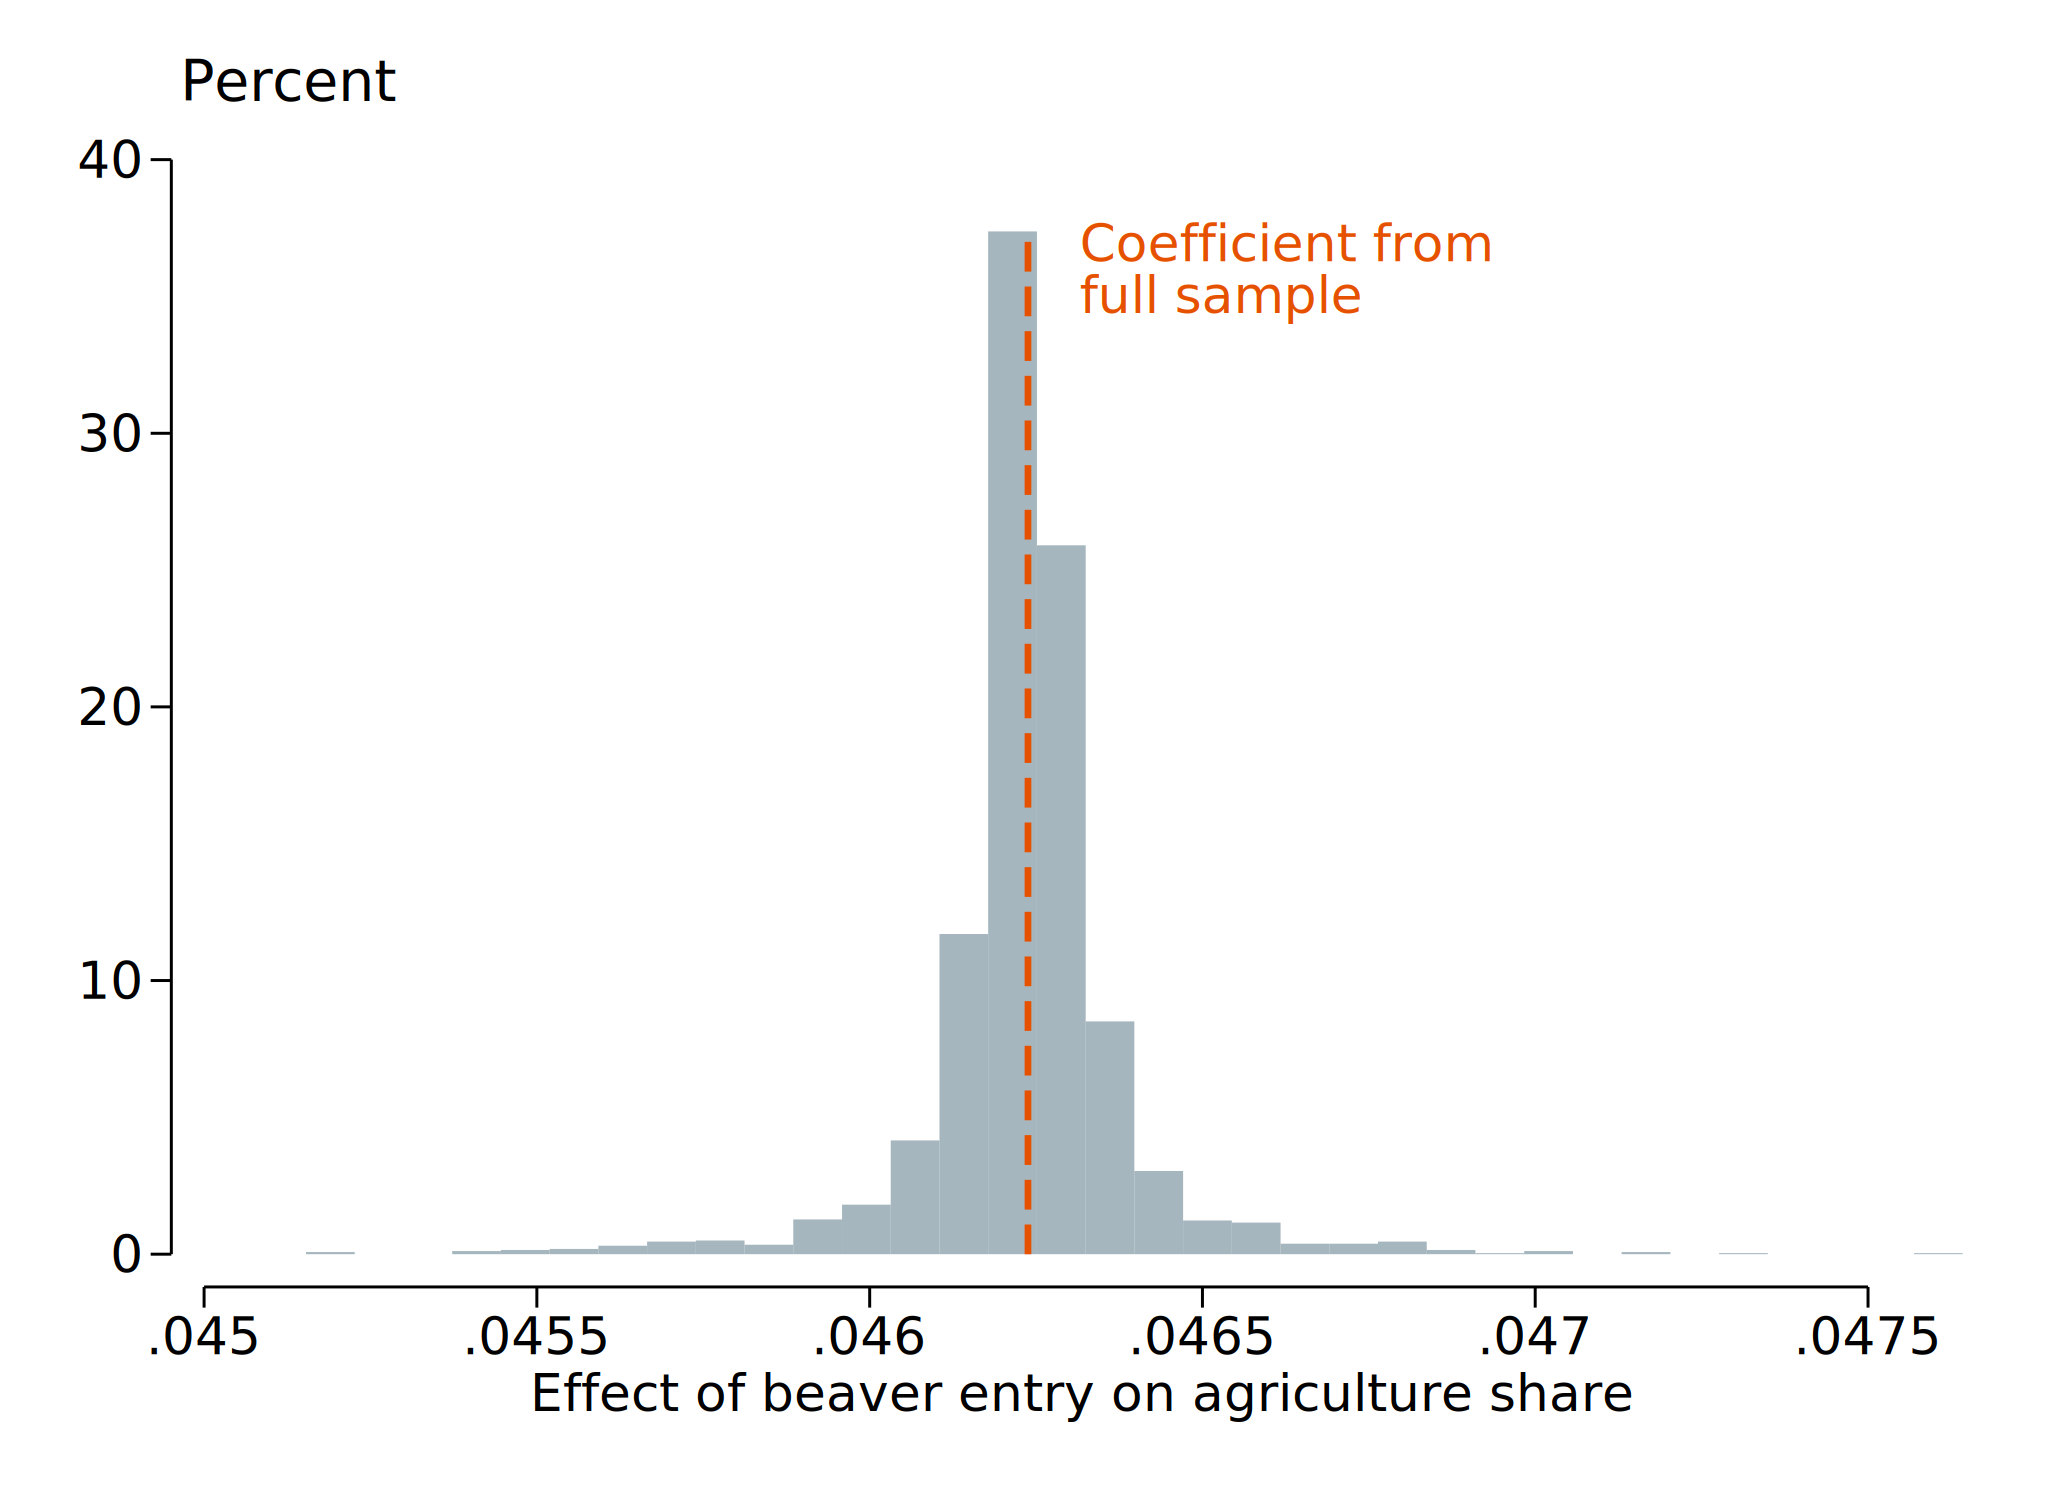
\includegraphics[width=0.7\linewidth]{output/figures/jackknife_distribution_Soverall_river_cells_AC.pdf}
    \caption*{\justifying \footnotesize Notes: The distribution of coefficients from a jackknife resampling exercise, where one landscape patch is left out each time, is plotted on the x-axis. Full sample specification is shown in Table \ref{table:beaver_sample_soil_Soverall_Cweather_controls}, column (4). }
    \label{fig:est-main-jackknife}
\end{figure}


% \input{appendix/additional_results.tex}

% \setcounter{page}{1}
% \setcounter{table}{0}
% \setcounter{figure}{0}
% \renewcommand{\thetable}{\thesection\arabic{table}}
% \renewcommand{\thefigure}{\thesection\arabic{figure}}
% \renewcommand{\thepage}{\thesection\arabic{page}}
% \renewcommand\thesection{\Alph{section}}
% \renewcommand\thesubsection{\thesection.\arabic{subsection}}
% \newpage
% \section{Data Construction}
% \input{appendix/additional_data.tex} 

\end{document}
